\phantomsection
\appendix
\addcontentsline{toc}{chapter}{Appendix}
\renewcommand{\thetable}{A.\arabic{table}}
\renewcommand{\thefigure}{A.\arabic{figure}}

\phantomsection
\section{Distribution of endpoint labels in the toxicity dataset}
\label{appendix:endpoint_labels}

\begin{table}[H]
\centering
\footnotesize
\csvautobooklongtable[table head=\caption{Distribution of endpoint labels in the entire toxicity dataset}\label{table:labels_tox}\\\hline
               \csvlinetotablerow\\\hline
               \endfirsthead\hline
               \csvlinetotablerow\\\hline
               \endhead\hline
               \endfoot,
			respect all]{include/tables/labels_tox.csv}
\caption*{Note: Labels after processing the toxicity tabular dataset. NA, not available in the toxicity dataset. Total compounds: 8975}
\end{table}

\begin{table}[h]
\centering
\footnotesize
\csvautobooklongtable[table head=\caption{Distribution of endpoint labels for the mass spectra collection}\label{table:labels_tox_MassBank}\\\hline
               \csvlinetotablerow\\\hline
               \endfirsthead\hline
               \csvlinetotablerow\\\hline
               \endhead\hline
               \endfoot,
			respect all]{include/tables/labels_tox_MassBank.csv}
\caption*{Note: NA, not available in the toxicity dataset. Total compounds: 1350}
\end{table}

%###################################################
\newpage
\phantomsection
\section{Cosine similarity and MS2DeepScore}
\label{appendix:Cosine similarity and MS2DeepScore}

\begin{table}[H]
\centering
\footnotesize
\csvautobooklongtable[table head=\caption{Frequency distribution of cosine score}\label{table:frequency_cosine}\\\hline
               \csvlinetotablerow\\\hline
               \endfirsthead\hline
               \csvlinetotablerow\\\hline
               \endhead\hline
               \endfoot]{include/tables/cosine_cumulative.csv}
\caption*{Note: Cosine scores of all unique pairs of the combined spectra. Tolerance cosine: 0.1 \textit{m/z}. 
x0 lower limit, x1 upper limit, f frequency, F cumulative frequency, rf, relative frequency, rF cumulative relative frequency, rf' inverse cumulative frequency, rF' inverse cumulative relative frequency.}

\end{table}

\begin{table}[H]
\centering
\footnotesize
\csvautobooklongtable[table head=\caption{Frequency distribution of MS2DeepScore}\label{table:frequency_ms2ds}\\\hline
               \csvlinetotablerow\\\hline
               \endfirsthead\hline
               \csvlinetotablerow\\\hline
               \endhead\hline
               \endfoot]{include/tables/ms2ds_cumulative.csv}
\caption*{Note: MS2DeepScore similarity score for all unique pairs of the combined spectra, 0.1 \textit{m/z} bin width. 
x0 lower limit, x1 upper limit, f frequency, F cumulative frequency, rf, relative frequency, rF cumulative relative frequency, rf' inverse cumulative frequency, rF' inverse cumulative relative frequency.}
\end{table}

%Moved

%Moved

%Moved

%Moved

%Moved

%Moved

%Moved

%Moved

%Moved

%Moved




\begin{figure}[h]
  \centering
	 \begin{subfigure}[a]{1\textwidth}
 		 \centering
  		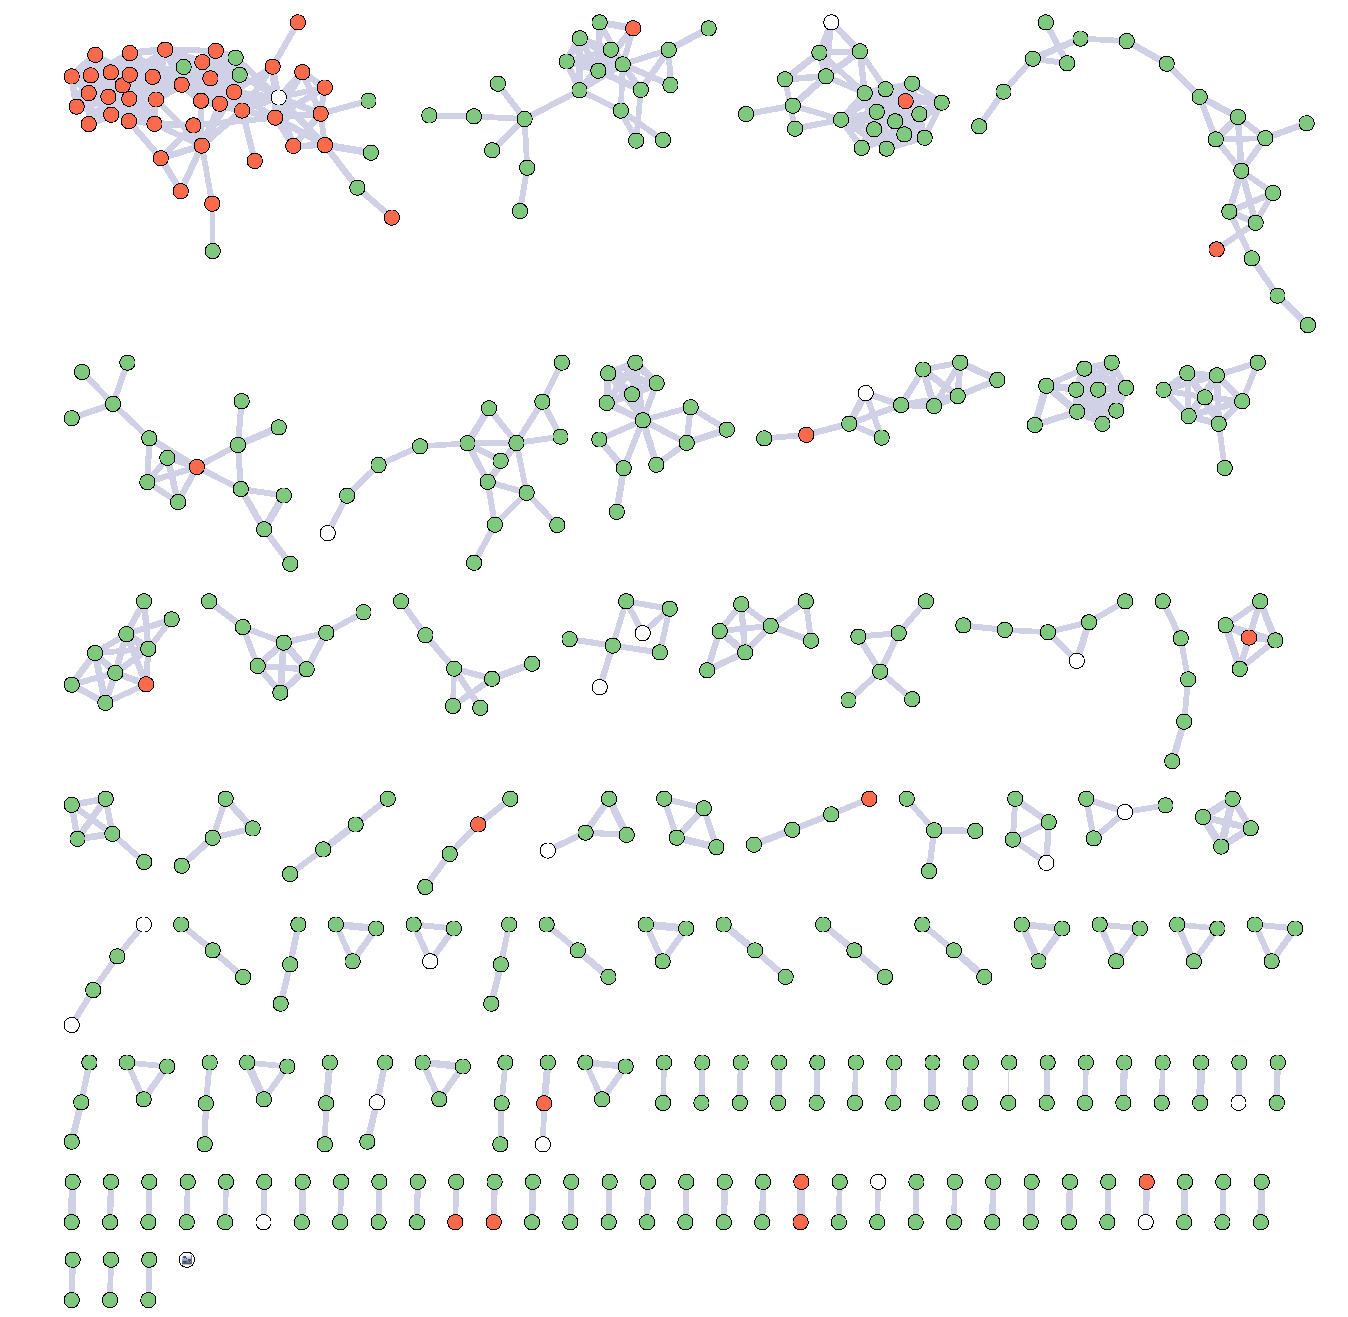
\includegraphics[width=0.7\textwidth]{include/img/net/NR.AR_MS2DeepScore.pdf}
 		 \caption{}
 	\end{subfigure}
 	\hfill
 		 \begin{subfigure}[a]{1\textwidth}
 		 \centering
 		 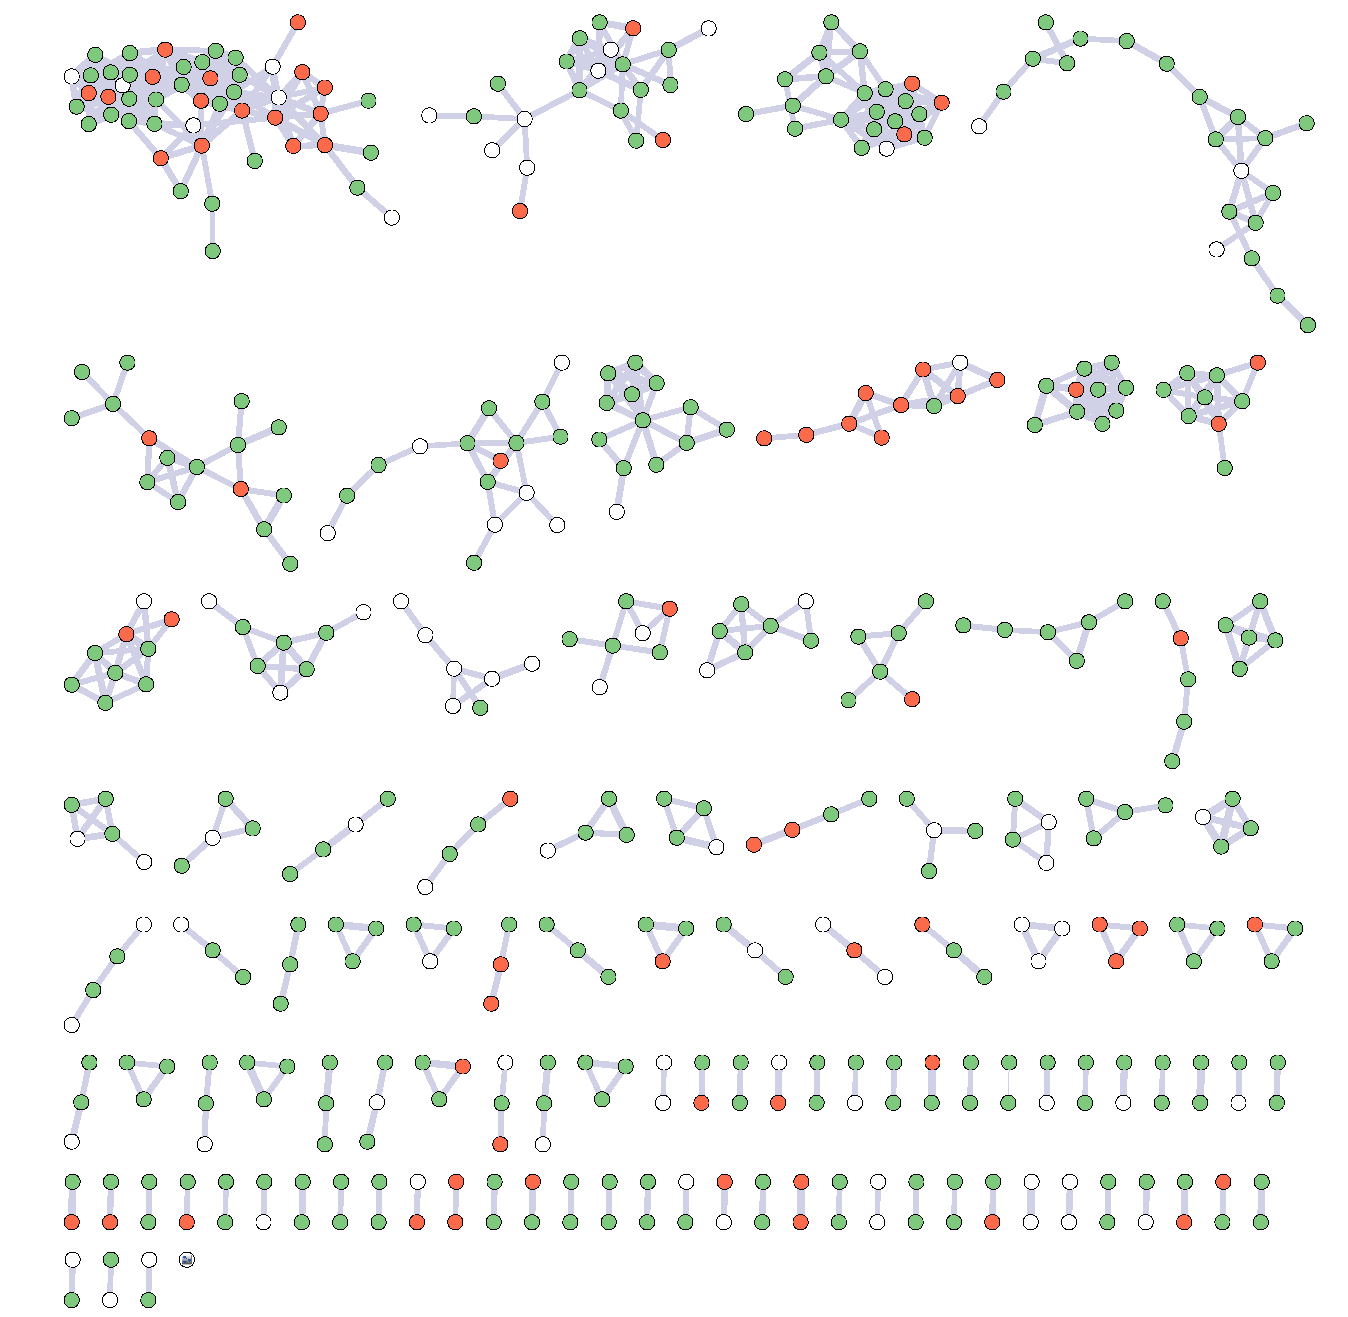
\includegraphics[width=0.7\textwidth]{include/img/net/NR.ER_MS2DeepScore.pdf}
 		 \caption{}
 	\end{subfigure}
  \caption{Spectral similarity network based on the MS2DeepScore similarity showing the (a) NR.AR and (b) SR.ARE endpoints. Nodes represent active (red), inactive (green) labels for the endpoints. Nodes in blank did not have a label. The edge width indicates the intensity of the score.}
  \label{fig:MS2DS_networks}
\end{figure}

%#############################################

\clearpage
\phantomsection
\section{\kNN{} cross-validation}
\label{appendix:k_CV}

\begin{figure}[h]
  \centering
	 \begin{subfigure}[b]{0.48\textwidth}
 		 \centering
 		 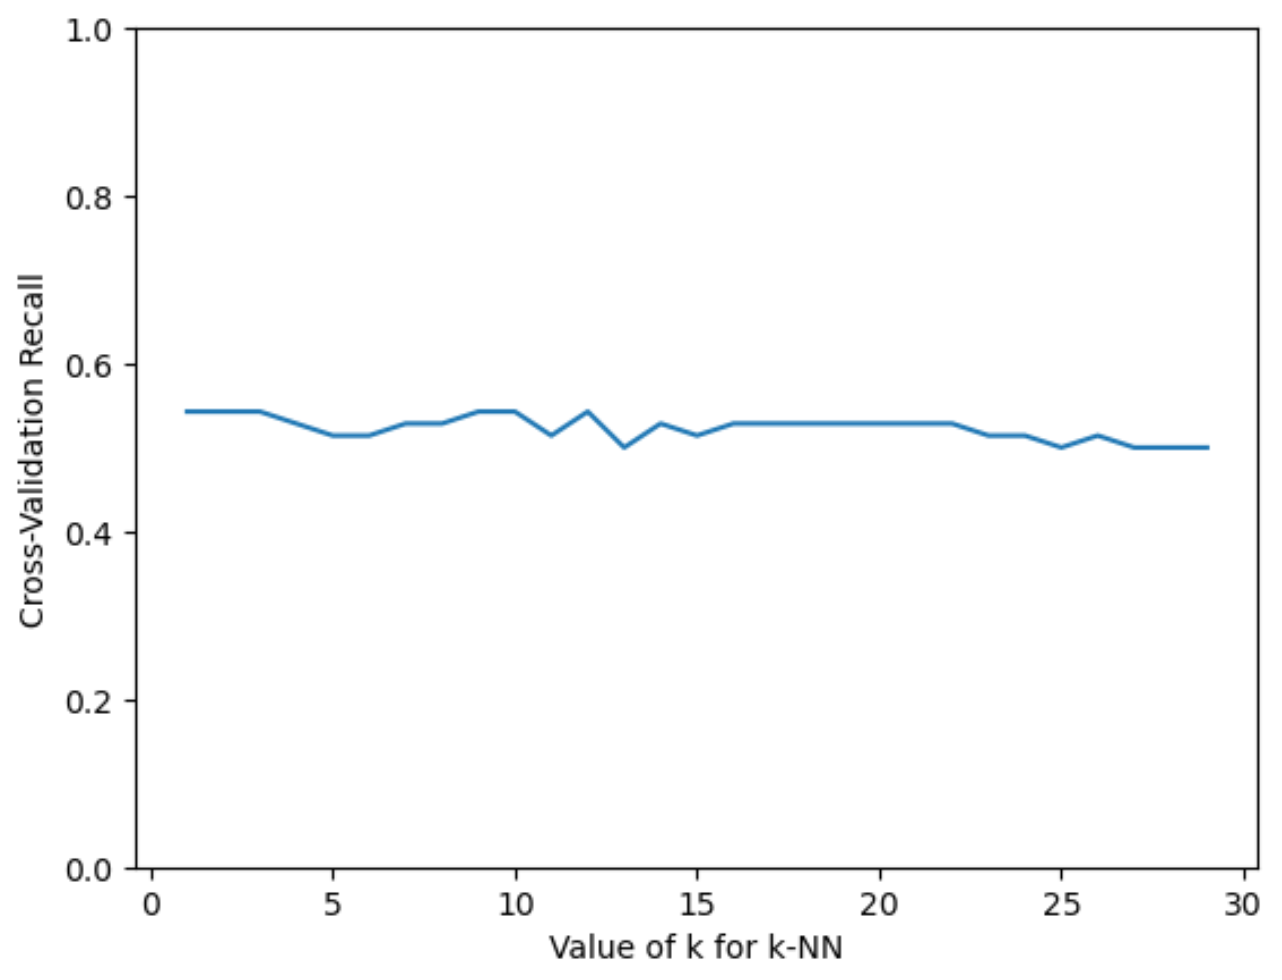
\includegraphics[width=\textwidth]{include/img/NR_AR_k.png}
 		 \caption{}
 	\end{subfigure}
 	\hfill
 		 \begin{subfigure}[b]{0.48\textwidth}
 		 \centering
 		 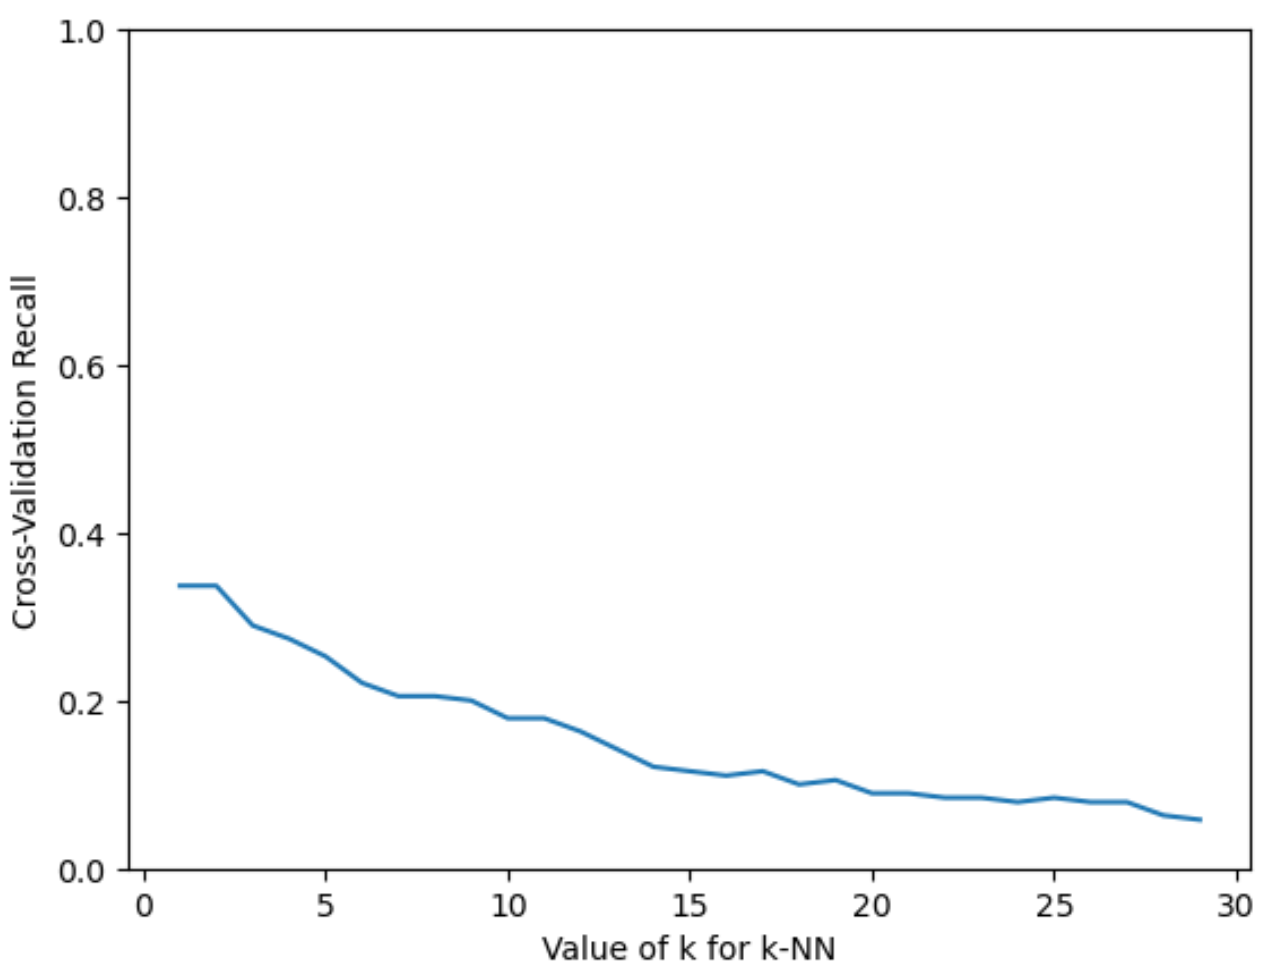
\includegraphics[width=\textwidth]{include/img/NR_AhR_k.png}
 		 \caption{}
 	\end{subfigure}
  \caption{(a) NR.AR and (b) NR.AhR recall for different values of \textit{k} for the \kNN{} algorithm with 5-fold cross-validation.}
  \label{fig:k_values}
\end{figure}



%#############################################

%Moved

%#############################################

\clearpage
\phantomsection
\section{Sample \tMS{} features}
\label{appendix:sample_details}

The tandem mass spectra from a wastewater sample was used to test the spectral network. The \tMS{} features were provided by Kruve Lab, Stockholm University. The sample has been collected from an effluent of a wastewater treatment plant in Stockholm in March 2022. Prior to the analysis, the sample has been stored at -20°C and filtered through a 0.45 \(\mu\)m filter. The measurement conditions are summarized in Table \ref{table:LC_sample} and \ref{table:HRMS_sample}. The data processing parameters for MS-DIAL (v. 4.80) are summarized in Table \ref{table:MS_DIAL}.

\begin{table}[htbp]
\centering
\footnotesize
\label{table:LC_sample}
\csvautobooklongtable[table head=\caption{Liquid chromatography conditions}\label{table:LC_sample}\\\hline
               \csvlinetotablerow\\\hline
               \endfirsthead\hline
               \csvlinetotablerow\\\hline
               \endhead\hline 	
               \endfoot,
			respect all, separator=semicolon]{include/tables/sample_specs/LC.csv}
\caption*{Source: Kruve Lab}

\end{table}


\begin{table}[htbp]
\centering
\footnotesize
\label{table:HRMS_sample}
\csvautobooklongtable[table head=\caption{HRMS measurement conditions}\label{table:HRMS_sample}\\\hline
               \csvlinetotablerow\\\hline
               \endfirsthead\hline
               \csvlinetotablerow\\\hline
               \endhead\hline
               \endfoot,
			respect all, separator=semicolon]{include/tables/sample_specs/HRMS.csv}
\caption*{Source: Kruve Lab}
\end{table}



\begin{table}[htbp]
\centering
\footnotesize
\csvautobooklongtable[table head=\caption{MS-DIAL processing parameters}\label{table:MS_DIAL}\\\hline
               \csvlinetotablerow\\\hline
               \endfirsthead\hline
               \csvlinetotablerow\\\hline
               \endhead\hline
               \endfoot,
			respect all, separator=semicolon]{include/tables/sample_specs/MS_DIAL.csv}
\caption*{Source: Kruve Lab}
\end{table}



%#############################################





%%%%%%%%%%%%%%%%%%%%%%%%%%%%%%%%%%%%%%%
%To skip \foreach in the compilation
%\iffalse

\clearpage
\phantomsection
\section{Spectral similarity networks with labels for all the endpoints}
\label{appendix:networks}
The selected spectral network for all endpoint labels is shown below. The spectral network uses a minimum cosine similarity of 0.6 and maximum number of edged from a node of 10. The active compounds are represented as nodes in red and the inactive ones in green. Nodes without color do not have activity information for the endpoint.

 \newcommand{\imagepath}{include/img/appendix/nets_endpoints/}
\newcommand{\imagelist}{NR.AhR.pdf, NR.AR.pdf, NR.AR.LBD.pdf, NR.Aromatase.pdf, NR.ER.pdf, NR.ER.LBD.pdf, NR.PPAR.gamma.pdf, SR.ARE.pdf, SR.ATAD5.pdf, SR.HSE.pdf, SR.MMP.pdf, SR.p53.pdf}
\foreach \filename in \imagelist {
\begin{figure}[H]
\centering
    \includegraphics[width=0.5\textwidth]{\imagepath\filename}
    \caption{\filename}
    \label{fig:\filename}
\end{figure}
}

%\fi
